\documentclass[12pt]{article}
\usepackage[left=1cm, right=1cm, top=2cm,bottom=1.5cm]{geometry} 

\usepackage[parfill]{parskip}
\usepackage[utf8]{inputenc}
\usepackage[T2A]{fontenc}
\usepackage[russian]{babel}
\usepackage{enumitem}
\usepackage[normalem]{ulem}
\usepackage{amsfonts, amsmath, amsthm, amssymb, mathtools}

\usepackage{fancyhdr}
\pagestyle{fancy}
\renewcommand{\headrulewidth}{1.5pt}
\renewcommand{\footrulewidth}{1pt}

\usepackage{graphicx}
\usepackage[figurename=Рис.]{caption}
\usepackage{subcaption}
\usepackage{float}

%%Наименование папки откуда забирать изображения
\graphicspath{ {./images/} }

%%Изменение формата для ввода доказательства
\renewcommand{\proofname}{$\square$  \nopunct}
\renewcommand\qedsymbol{$\blacksquare$}

\addto\captionsrussian{%
	\renewcommand{\proofname}{$\square$ \nopunct}%
}
%% Римские цифры
\newcommand{\RN}[1]{%
	\textup{\uppercase\expandafter{\romannumeral#1}}%
}


\theoremstyle{definition}
\newtheorem{defn}{Опр:}
\newtheorem{rem}{Rm:}
\newtheorem{prop}{Утв.}
\newtheorem{exrc}{Упр.}
\newtheorem{lemma}{Лемма}
\newtheorem{theorem}{Теорема}
\newtheorem{corollary}{Следствие}

\newenvironment{cusdefn}[1]
{\renewcommand\thedefn{#1}\defn}
{\enddefn}



\DeclareRobustCommand{\divby}{%
	\mathrel{\text{\vbox{\baselineskip.65ex\lineskiplimit0pt\hbox{.}\hbox{.}\hbox{.}}}}%
}


\newcommand{\smallerrel}[1]{\mathrel{\mathpalette\smallerrelaux{#1}}}
\newcommand{\smallerrelaux}[2]{\raisebox{.1ex}{\scalebox{.75}{$#1#2$}}}

\newcommand{\smallin}{\smallerrel{\in}}
\newcommand{\smallnotin}{\smallerrel{\notin}}


\begin{document}
	\lhead{Математический анализ - I}
	\chead{Шапошников С.В.}
	\rhead{Лекция - 1}
\section*{Множества}

\begin{defn}
	\uwave{Множество} - это набор, совокупность, собрание объектов, которые называются \uwave{элементами множества}.
\end{defn}

$A$ - множество, $a \in A$ - ``$a$ принадлежит $A$'', $a \notin A$ - ``$a$ не принадлежит $A$''.

Как задавать множества? Есть несколько способов:
\begin{enumerate}[label={(\arabic*)}]
	\item \uwave{Перечисление}: $\{a_1, a_2, a_3, ...\}$;
	\item \uwave{Указание свойства}: $\{\,x \colon x^2 =1 \,\}$ - задавать так, не очень безопасно;
\end{enumerate}

\subsection*{Парадок Рассела}

Пусть $K$ - набор множеств, которые \textbf{не} содержат себя в качестве элемента.
Например, $\{1, 3\} \in \{1, 3, \{1,3\}\}$. Верно ли, что $K \in K$?

\textbf{Предположим, что да} $\Rightarrow$ это будет противоречить определению набору множеств $K$ - получили противоречие.

\textbf{Предположим, что нет} $\Rightarrow K \notin K \Rightarrow$, но по определению $K \in K$ - получили противоречие.

Таким образом, корректно выделять часть множества. Множество всех множеств будет противоречить аксиоматике $ZF$.

Для детей обычно дают парадокс брадобрея: брать только тех, кто себя не бреет.

\subsection*{Аксиоматика Цермело-Френкеля (ZF)}

Более подробно - см. Зорич В.А. (I-II том).

\begin{defn}
	$\varnothing$ - пустое множество: про всякий объект можно утверждать, что он этому множеству не принадлежит.
\end{defn}

$\{\,x \colon x \neq x\,\}$, может есть несколько $\varnothing$? Используя $ZF \Rightarrow \varnothing$ - единственно.

\begin{defn}
	\uwave{Включение} $A \subset B$, $A$ является подмножеством $B$, если $\forall a \in A \Rightarrow a \in B$
\end{defn}  

\subsection*{Свойства:}
	
	\begin{enumerate}[label={(\arabic*)}]
		\item $A \subset A$;
		\item $A \subset B,\, B \subset C \Rightarrow A \subset C$;
	\end{enumerate}

\begin{defn}
	\uwave{Равенство множеств} $A = B$ выполняется, если одновременно $A \subset B$ и $B \subset A$.
\end{defn}

\begin{prop}
	$\varnothing \subset A$, $\forall A$
	
	\begin{proof}{\uwave{(От противного)}:}
		Пусть не выполняется $(a \in \varnothing \Rightarrow a \in A) \Rightarrow \exists a \in \varnothing$ и $a \notin A$ это невозможно, так как в $\varnothing$ нет элементов.
	\end{proof}
\end{prop}

\newpage

\section*{Множество натуральных чисел}

$\mathbb{N} = \{1, 2, 3, ... \,, n, ...\}$ - не знаем как получается, пока берем аксиоматически.

\subsection*{Аксиомы Пеано:}
\begin{enumerate}
	\item $\forall n \in \mathbb{N}$, $\exists!$ элемент, который называется \uwave{следующим} и обозначается $n+1$;
	\item $\exists!$ элемент, который ни за кем не следует и называется \uwave{единицей} и обозначается 1;
	\item $\forall$ элемента отличного от 1, $\exists!$ элемент за которым он следует (\uwave{единственный предыдущий});
	\item \textbf{(Аксиома индукции)}: Если $M \subset \mathbb{N}\colon 1 \in M$ и $\forall n \in M \Rightarrow (n+1) \in M$, то $M = \mathbb{N}$;
\end{enumerate}

Следует заметить, что аксиомы 1-3 запрещают следующее поведение натуральных чисел:
\begin{figure}[H]
	\centering
	\begin{subfigure}[b]{0.33\textwidth}
		\centering
		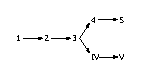
\includegraphics[width=4cm, height = 2cm]{1_1}
		\label{fig:1_1}
	\end{subfigure}
	\begin{subfigure}[b]{0.32\textwidth}
		\centering
		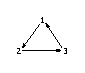
\includegraphics[width=2cm, height = 2cm]{1_2}
		\label{fig:1_2}
	\end{subfigure}
	\begin{subfigure}[b]{0.33\textwidth}
		\centering
		\includegraphics[width=4cm, height = 2cm]{1_3}
		\label{fig:1_3}
	\end{subfigure}	
	\caption{Последовательности не удовлетворяющие аксиомам 1-3}
	\label{fig:Сюръективность}
\end{figure}

Но при этом, если не использовать аксиому 4, то возможна следующая последовательность: $$\{1, 2, 3, \dotsc; \RN{1}, \RN{2}, \RN{1}, \RN{2}, \RN{1}, \dotsc\}$$
таким образом, 4-ая аксиома делает данное множество - наименьшим.

\subsection*{Метод математической индукции}

$A_1, A_2, A_3, \dotsc$ - утверждения. Хотим доказать, что все $A_k$ - истинны.

$\left.\begin{aligned}
&	A_1 \text{ - истина  (База)}\\
&	\forall n,\, A_n \Rightarrow A_{n+1} \text{(Шаг)}   
\end{aligned}
\right\}
\Rightarrow \text{ все } A_n \text{ - истинные}$.

\begin{theorem}
	Аксиома индукции $\Rightarrow$ Метод математической индукции
\end{theorem}
\begin{proof}
	Пусть $M = \{\,n \colon A_n \text{ - истина}\,\}$. \\
	\uline{База}: $1 \in M$\\
	\uline{Шаг}: $\forall n,\, n \in M \Rightarrow (n+1) \in M \Rightarrow$ по АИ $M = \mathbb{N} \Rightarrow$ все $A_n$ - истинные $\Rightarrow$ ММИ выполняется. 
\end{proof}

\begin{theorem}
	\textbf{(Неравенство Бернулли)}: $\forall n \in \mathbb{N}$, $x \geq -1 \Rightarrow (1+x)^n \geq 1 + nx$
\end{theorem}

\begin{proof}
	Используя метод математической индукции:\\
	\uline{База}: $n = 1,\, (1+x) \geq 1 + x$ - верно.\\
	\uline{Шаг}: предположим, что для $n$ - верно, $(1 + x)^n \geq 1 + nx$, тогда\\
	
	$(1+x)^{n+1} = (1+x)^n(1+x) \underset{\text{т.к. } (1+x)\geq 0}{\geq} (1 + nx)(1 + x) = 1 + x + nx + \underbrace{nx^2}_{\geq 0} \geq (1 + (n+1)x)$
\end{proof}

\begin{rem}
	Можно доказать и для $x \geq -2$, но не через индукцию.
\end{rem}

\subsection*{Бином Ньютона}

Определим число сочетаний $C_n^k$ - количество способов выбрать из $n$ объектов - $k$ объектов или выбрать из $n$ - элементного множества $k$ - элементное.\\
$n$ человек, сколькими способами можно назначить $k$ человек ? $\Rightarrow C_n^k$: 1-ый человек - $n$ способов, 2-ой человек - $(n-1)$ способ, $\dotsc$, k-ый человек - $(n-k+1)$ способ $\Rightarrow n\cdot  (n-1) \cdot (n-2) \cdot \dotsc \cdot (n-k+1)$, но так как порядок не важен, то делим это число на число перестановок $\Rightarrow \dfrac{1}{k!}\cdot n\cdot(n-1)\cdot\dotsc\cdot(n-k+1)$, где $k!$ - число перестановок на $k$ элементов.

\begin{theorem}
\textbf{(Бином Ньютона)}: $(a+b)^n = \sum\limits_{k = 0}^n C_n^k a^kb^{n-k}$, где $C_n^k = \dfrac{n!}{k!(n-k)!}$, $n! = 1\cdot2\cdot3\cdot \dotsc \cdot n$, $0! = 1$.
\end{theorem}
\begin{proof}\hfill
	
	\textbf{(\RN{1}) способ:} $(a+b)^n = \overbrace{(a+b) \dotsc (a+b)}^{n \; \text{штук}} = \dotsc a^kb^{n-k}$ так как идет перемножение скобок, то $k + (n-k) = n$, выбираем скобки, где будет $a$, из оставшихся берем $b \Rightarrow C_n^k a^k b^{n-k} \Rightarrow (a+b)^n = \dotsc C_n^k a^k b^{n-k}$. Индукция в таком способе - в перемножении.\\
	
	\textbf{(\RN{2}) способ:} используем ММИ \\
	\uline{База}: $n = 1,\, (a+b) = C_1^0 b + C_1^1 a = a + b$ - верно.\\
	\uline{Шаг}: предположим, что для $n$ - верно $\Rightarrow$ 
	$$(a+b)^{n+1} = (a+b)^n(a+b) = \big(\sum\limits_{k=0}^nC_n^ka^kb^{n-k}\big)(a+b)$$ таким образом получим слагаемые вида: 
	
	$a\cdot \big(\sum\limits_{k=0}^nC_n^ka^kb^{n-k}\big) = \sum\limits_{k=0}^nC_n^ka^{k+1}b^{n-k}$ и $b\cdot \big(\sum\limits_{k=0}^nC_n^ka^kb^{n-k}\big)) = \sum\limits_{k=0}^nC_n^ka^kb^{n-k+1}$, все они будут иметь вид $$\dotsc a^mb^{n+1-m}\text{, где }m = 0,\dotsc, n+1 \Rightarrow $$  
	$C_n^ka^{k+1}b^{n-k} = (C_n^{m-1} a^{m-1})ab^{n-m+1}, m = 1,\dotsc, n+1$ и $C_n^ka^kb^{n-k+1} = C_n^ma^m(b^{n-m}b), m = 0,\dotsc,n \Rightarrow$
	
	Поскольку $\frac{n!}{(m-1)!(n-m+1)!} + \frac{n!}{m!(n-m)!} = n!\cdot \frac{m + n - m + 1}{m!(n-m+1)!} = \frac{(n+1)!}{m!(n-m+1)!} = C_{n+1}^m$, то
	
	$C_n^{m-1}a^mb^{n-m+1} + C_n^m a^mb^{n-m+1} = C_{n+1}^m a^m b^{n-m+1}$, где $m = 0, 1, \dotsc, n+1 \Rightarrow (a+b)^{n+1} = \sum\limits_{m = 0}^{n+1}C_{n+1}^m a^m b^{n-m+1}$
\end{proof}

\end{document}